\chapter{Reading the height from the network's own current}\label{ch:height}

MAGIC-UNet is never told the standoff. But it outputs a current, and a current implies a height. This chapter shows how
to read it out, where that works, and where it fails. It is milestone M1a of the review.

\section{The idea}

Chapter~\ref{ch:magic} showed that from a sheet current $J$, exact physics gives the field at \emph{any} height. So try
every height. For each trial height $h$, compute the field that the predicted current would produce there, and compare
it with the field that was actually measured:
\[
\text{misfit}(h)=\text{mean over } B_x, B_y, B_z \text{ of }\ \frac{\|\,\text{forward}(J,h)-b\,\|}{\|b\|},\qquad
h^\ast=\arg\min_h\ \text{misfit}(h).
\]
The height with the smallest misfit is the read-out $h^\ast$. Nothing is trained for this. It is a fit with one
parameter.

\begin{figure}[H]
\centering
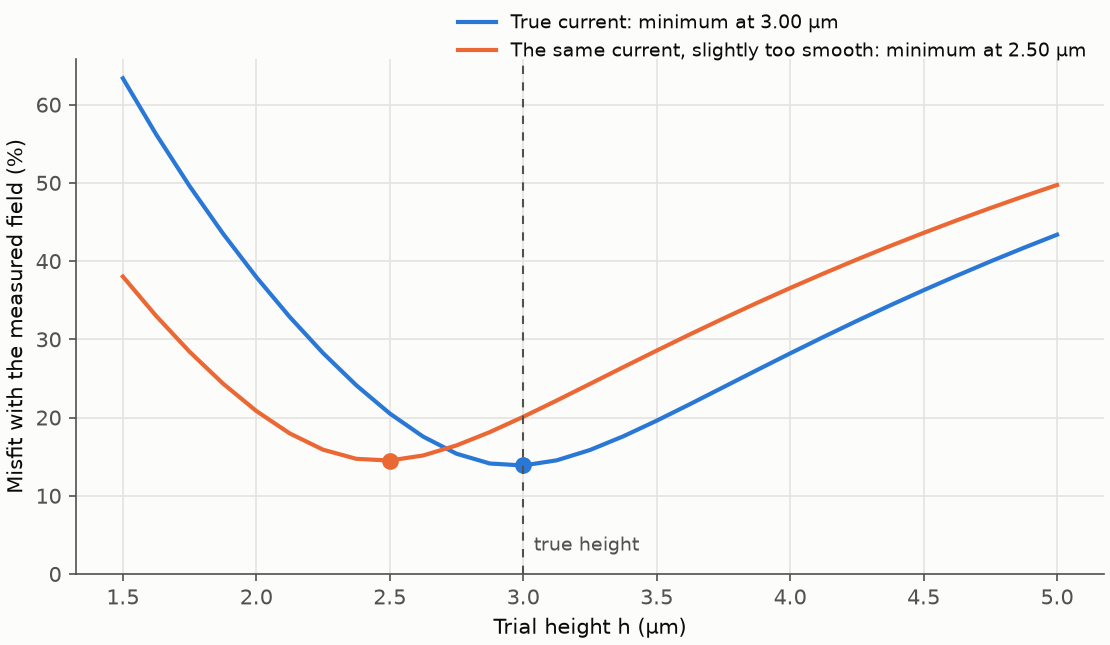
\includegraphics[width=0.8\textwidth]{late_height_misfit}
\caption{The read-out on one simulated layout measured at 3\um. With the true current the misfit has its minimum exactly
at 3\um. With the same current slightly smoothed, the minimum moves to a smaller height.}
\label{fig:late_height}
\end{figure}

\section{The code}

The Fourier transform of the current is the expensive part, and it does not depend on the height. So it is done once:

\begin{code*}{m12_common.py}
    fx, fy = np.fft.rfft2(jx), np.fft.rfft2(jy)
    fz = 1j * (wy * fx - wx * fy) / safe
    return (fx, fy, fz), k, (ny, nx)
\end{code*}

These are the same three lines as the Biot--Savart step of Chapter~\ref{ch:magic}. Then each trial height only needs
one multiplication by $e^{-kh}$ and one inverse transform:

\begin{code*}{m12_common.py}
    decay = 0.5 * mu0_ut * np.exp(-k * height)
    return np.stack([np.fft.irfft2(f * decay, s=shape)[pad:pad + image, pad:pad + image]
                     for f in spectra])
\end{code*}

\begin{code*}{m12_common.py}
    return np.array([relative_l2(field_at(spectra, k, shape, h, image, pad), b).mean()
                     for h in heights])
\end{code*}

The search is done in two passes: a coarse grid in steps of 0.1\um, then a fine grid in steps of 0.01\um\ around the
best coarse value.

\begin{code*}{m12_common.py}
    coarse = misfit_fn(grid)
    h0 = grid[int(np.argmin(coarse))]
    fine_h = np.round(np.arange(h0 - FINE_HALF, h0 + FINE_HALF + 1e-9, FINE_STEP), 3)
\end{code*}

\begin{code*}{m12_common.py}
    edge = bool(h <= lo + 0.1 or h >= h_max - 0.1)
\end{code*}

The last line is a warning flag. If the minimum sits at the end of the grid, the true minimum may lie outside it, and
the result should not be trusted.

A test on the Mac checks the whole thing with a known answer: it builds fields at 1.37, 3.00 and 6.42\um\ from a known
current and recovers each height to 0.01\um. On the server the same computation runs on the GPU:

\begin{code*}{m1_rescore.py}
def read_height(sheet, b, device, h_max=mc.EDGE[1]):
    b32 = torch.as_tensor(np.asarray(b, np.float32), device=device)
    b_norm = (b32 ** 2).sum((-2, -1)).sqrt()
    return mc.read_height(lambda hs: sheet.misfit(hs, b32, b_norm), h_max)
\end{code*}

\section{Why the read-out can be wrong}

Look again at Figure~\ref{fig:late_height}. The orange curve uses a current that is slightly too smooth. Its minimum is
at a \emph{smaller} height. This is the ambiguity of Chapter~\ref{ch:question}, seen from the other side: a smoother
source closer to the sensor gives the same field as a sharper source further away. So:
\begin{itemize}
\item a predicted current that is \textbf{too smooth} reads the height \textbf{too low};
\item a predicted current that is \textbf{too sharp} or too strong reads it \textbf{too high}.
\end{itemize}

\begin{keyidea}[The read-out measures the network, not only the height]
$h^\ast$ is the height at which \emph{this network's current} best explains the data. If the current is right, $h^\ast$ is
the true height. If the current is biased, $h^\ast$ is biased in the matching direction.
\end{keyidea}

\section{On simulation}

50 validation layouts at each standoff, where the truth is known:

\begin{center}
\small
\begin{tabular}{lcccccccc}
\toprule
True standoff (\textmu m) & 1 & 2 & 3 & 4 & 5 & 6 & 8 & 10 \\
\midrule
Run 2, median $h^\ast$ & 1.21 & 2.05 & 3.06 & 4.01 & 4.46 & 4.43 & 3.66 & 2.63 \\
Run 3, median $h^\ast$ & 1.18 & 2.11 & 3.12 & 4.14 & 5.29 & 6.50 & 8.27 & 7.84 \\
\bottomrule
\end{tabular}
\end{center}

\begin{itemize}
\item \textbf{Run 2} reads the height well from 1.5 to 4\um\ (median error 2--5\%). That is its training range. Above it,
the read-out stops following and falls back toward 3--4\um: the network keeps drawing currents that belong to its
training heights.
\item \textbf{Run 3} follows the truth from 1.5 to 8\um: within 15\% for 93\% of images, reading about 5\% high. It fails at
both ends of its range, 1 and 10\um.
\end{itemize}

This is what the one-sided ambiguity predicts: the prior decides the height, so a network knows heights only where it
has learned what sources look like at those heights.

\section{On COMSOL}

At 3\um\ on COMSOL, run 2 reads 2.93--3.01\um\ on all five configurations. Outside 3\um\ it is pulled toward 3: an input
at 2\um\ reads 2.32, and at 4\um\ reads 3.61. Run 3 reads the C1-family coils at 2.97--3.10\um, and \code{IC_4um} at
3.86\um, too high. That fits Chapter~\ref{ch:run3}: on that coil its current is too strong, and a too-strong current
reads high.

One more observation, to be picked up later. On COMSOL \code{L1_C1} at large standoffs, run 3 reads \emph{low}: 6.26 at
7\um, 7.97 at 10\um. On simulation it reads high there. Chapter~\ref{ch:ten_results} finds the reason.

\section{The test that failed}

The review predicted: run 3 fails on the IC coil because each tile picks its own height, so imposing one global height
should rescue it. Under the protocol, that was a decision rule written in advance. The result:

\begin{center}
\begin{tabular}{lc}
\toprule
Run 3 on \code{IC_4um}, 3\um\ to 0.5\um & Error \\
\midrule
Raw & 52.0\% \\
Corrected at its own read-out, 3.86\um & 46.9\% \\
Corrected at the true height, 3\um & 37.3\% \\
Run 2, raw, for comparison & 29.6\% \\
\bottomrule
\end{tabular}
\end{center}

(``Corrected'' is the step of the next chapter.) Even with the true height it stays far from run 2. So the prediction
was wrong, and the review says so.

\begin{keyidea}[The lesson for any future method]
The per-tile decision is baked into the predicted current. A height applied afterwards cannot undo it. A real height
search must \emph{re-run the reconstruction} at each candidate height, and not re-project one prediction. The read-out is
a cheap shortcut, and this experiment showed where the shortcut ends.
\end{keyidea}

\begin{defend}[If your professor asks: does your method estimate the standoff?]
It reads one from the network's own current, with no extra training: within a few per cent inside the range the
network was trained on, on simulation, and 2.93--3.01\um\ at a true 3\um\ on COMSOL. It is not an independent
measurement. It inherits the network's bias, as the IC coil shows, and it has no uncertainty attached yet.
\end{defend}
